\section{Discussion} 
In this chapter, we will review the results of number of constituent quark scaling of elliptic for identified particles from STAR BES-I and compare with the results that from 3 GeV to discuss the partonic collectivity at RHIC-STAR energy region.  The $p_{T}$ integrated $v_{2}$ will also be discussed and compared with world data. The excitation function indicates the elliptic flow evolves from a in-plane flow ($v_{2} > 0$) to an out-of-plane flow pattern as the collision energy decreases due to the shadowing effect from spectators. The directed flow slope of identified particle will be discussed and compared with the higher energy from STAR BES-I. 

\subsection{Development of elliptic flow}
In non-central heavy ion collisions, the overlap region of colliding nuclei is like almond-shaped. This spatial anisotropy will cause larger pressure gradients in the direction of participant plane compared to out of this plane, which finally result in azimuthal anisotropy of the momenta of the produced particles. The elliptic flow $v_{2}$ is the second harmonic coefficient of the Fourier decomposition of the azimuthal particle distribution with respect to event plane.

At high energy, the passage time of the projectile and target spectators is much smaller than the development time of medium expansion. The passage time is $ \sim 2R/(\gamma_{0} v_{0})$, where R is the nuclear radius, $v_{0}$ is the spectator velocity in the CM frame. The development time of medium expansion can be estimated as $\sim$ $R/c_{s}$, where the speed of sound $c_{s} = \sqrt{\partial p/\partial e}$, where the p is the pressure, and e is the energy density. The spectators will have little effect on the medium expansion at high energy. When the collision energy decreases, the passage time of spectators might be larger than the development time of medium expansion. This will cause shadowing of "squeeze-out" effect by spectators. It means the spectators shadow the expansion of medium alone impact parameter direction, which leads to negative elliptic flow \cite{Pinkenburg:1999ya}. This is important for understanding the equation of state (EoS) at low energy \cite{Danielewicz:1998vz, Danielewicz:2002pu}.

\subsection{Number of constituent quark scaling of elliptic flow ($v_{2}$)}
Quark coalescence and recombination mechanisms ~\cite{Fries:2003vb,Hwa:2003bn} in particle production for heavy-ion collisions predict that if particles are made up of quarks then the elliptic flow $v_{2}(p_{T})$ of the particles will scale with their number of constituent quarks and follow a universal trend ~\cite{Molnar:2003ff} . The number of constituent quark for meson is two, for baryon is three. It is always performed as $v_{2}$ divide by number of consistent quark ($n_{q}$) for various particle species as a function of $(m_{T}-m_{0})/n_{q}$. Here the transport mass $m_{T}$ is defined as $m_{T} = \sqrt{p_{T}^{2}+m_{0}^{2}}$. The variable transverse kinetic energy is chosen in order to remove particle mass dependence from the flow coefficients.  The number of constituent quark scaling for elliptic flow has been argued for a evidence for partonic degree of freedom.

From STAR previous measurements, the identified hadrons follow a universal scaling at top BES-I energy 200 GeV, which indicates the light quark (u, d, s) even charm quark (c) exhibit the same strong collective behavior and may be close to thermal equilibrium in Au+Au collisions at 200 GeV ~\cite{Abelev:2008ae, Adamczyk:2015ukd, Adamczyk:2017xur}. While at lower STAR BES-I energy region, the difference of elliptic flow between particle and anti-particle have been observed, especially for the baryons. The difference is increasing with collision energy decreasing ~\cite{Adamczyk:2013gv}. This indicates the break of NCQ scaling between particles and antiparticles. Many theoretical calculation or transport model ~\cite{Dunlop:2011cf, Steinheimer:2012bn, Sun:2014rda, Hatta:2015era, Xu:2013sta} study this effect and have a description of pion, kaon and proton $v_{2}$ difference. The individual positive and negative charged hadrons still have good NCQ scaling when collision energy is larger than 19.6 GeV \cite{Adamczyk:2013gw}. At 7.7 GeV, we still have NCQ scaling within 10\% uncertainty. From STAR recent publication, the pion and proton $v_{2}$ follow same trend within statistics errors at 4.5 GeV~\cite{Adam:2020pla}. We would like to ask whether the partonic phase developed and how the NCQ scaling behave at $\sqrt{s_{NN}}$ = 3 GeV.

Fig \ref{fig:v2pt_ncq} shows the number of constituent scaled $v_{2}$ as a function of transverse kinetic energy in 10-40\% centrality. The data points are from STAR run18 54.4GeV and FXT 3GeV, and run19 27GeV, pion, kaon, proton $v_{2}$ results. The different color dash lines represent the fit to data from 200-3 GeV, in order to strength the scaled $v_{2}$ at different energy \cite{Dong:2004ve}, they can be found in Figure\ref{fig:v2pt_ncq_fit}. As we can see at 27 and 54.4 GeV, the NCQ scaling of individual positive and negative particles holds well, which is consistent with that the elliptic flow is driven by partonic collectivity. While at 3 GeV, we found different behavior of $v_{2}$. By comparing to the data from 4.5 GeV, we found the measured $v_{2}$ for all particles are negative and the NCQ scaling is absent, especially for positive charged particles. This significant change from 4.5GeV to 3GeV indicates new medium properties produced at 3GeV that are different from the partonic matter created in high energy collisions. 

\begin{figure}[h]
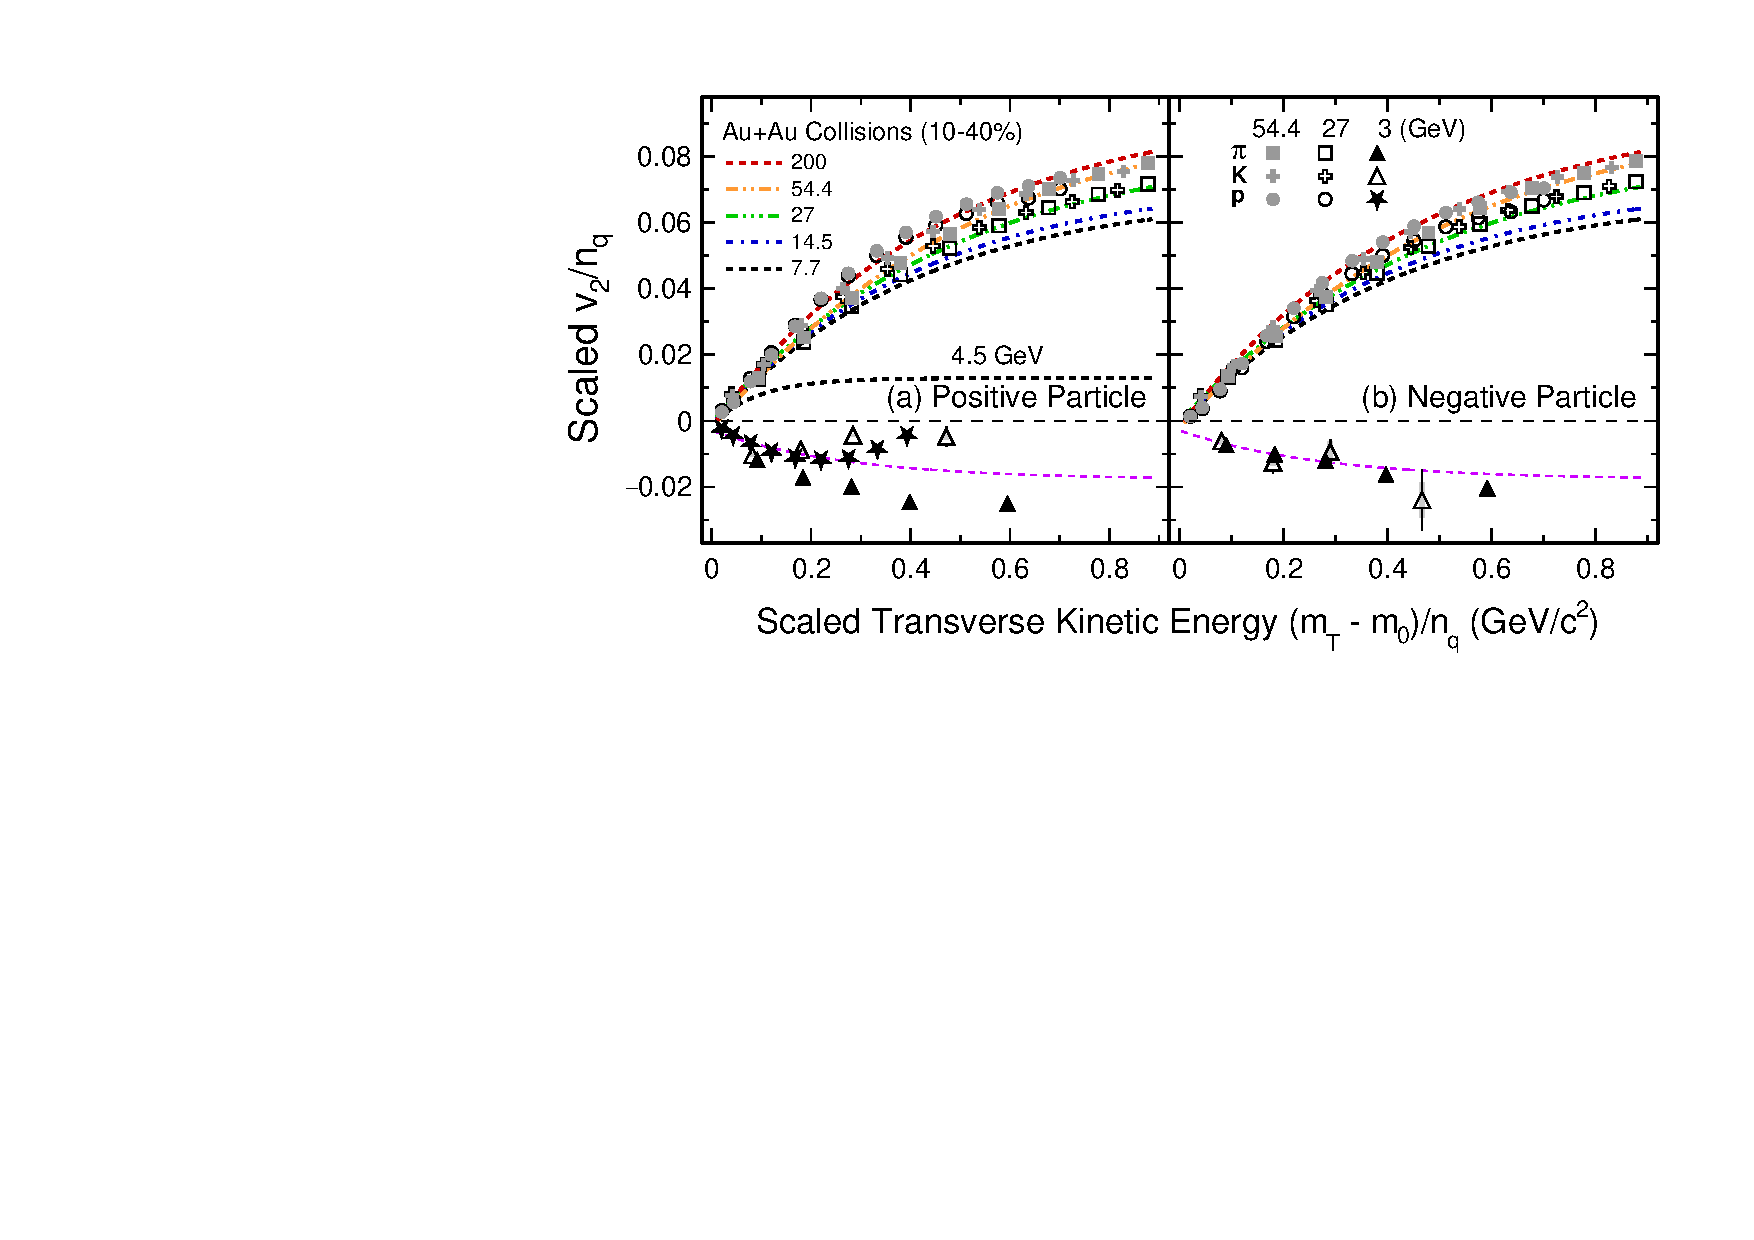
\includegraphics[scale=0.6]{FXT3gev/chapter4/fig/v2pt_ncq.pdf}
\caption{Number of constituent quark scaled $v_{2}$ for pion, kaon and proton as a function of scaled transverse kinetic energy in 10-40\% at 3, 27 and 54.4 GeV for positive charged particles (a) and negative charged particles (b). Different color dash line indicates the strength of scaled $v_{2}$ at different collision energy from fitting.}
\label{fig:v2pt_ncq}
\end{figure}

\begin{figure}
    \centering
    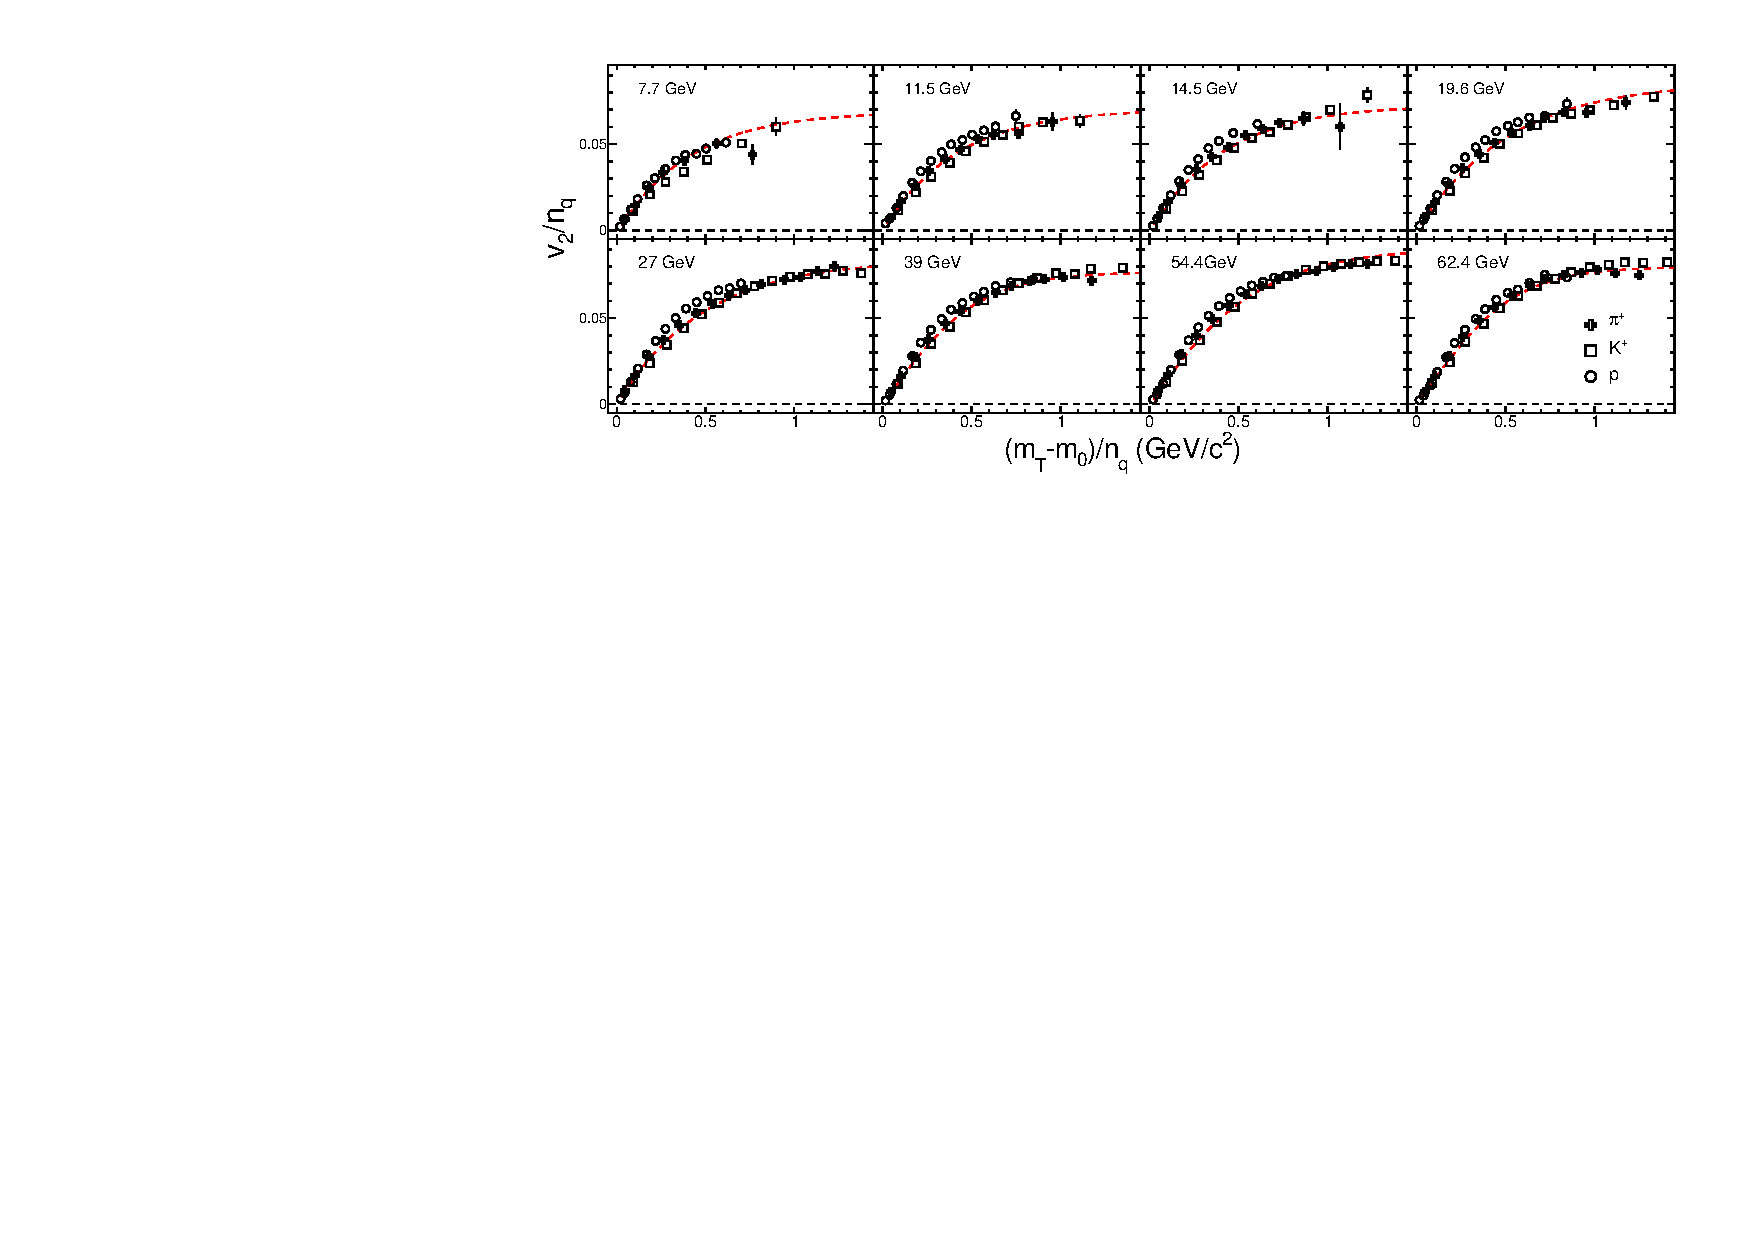
\includegraphics[scale=0.7]{FXT3gev/chapter4/fig/v2ncq_energy.pdf}
    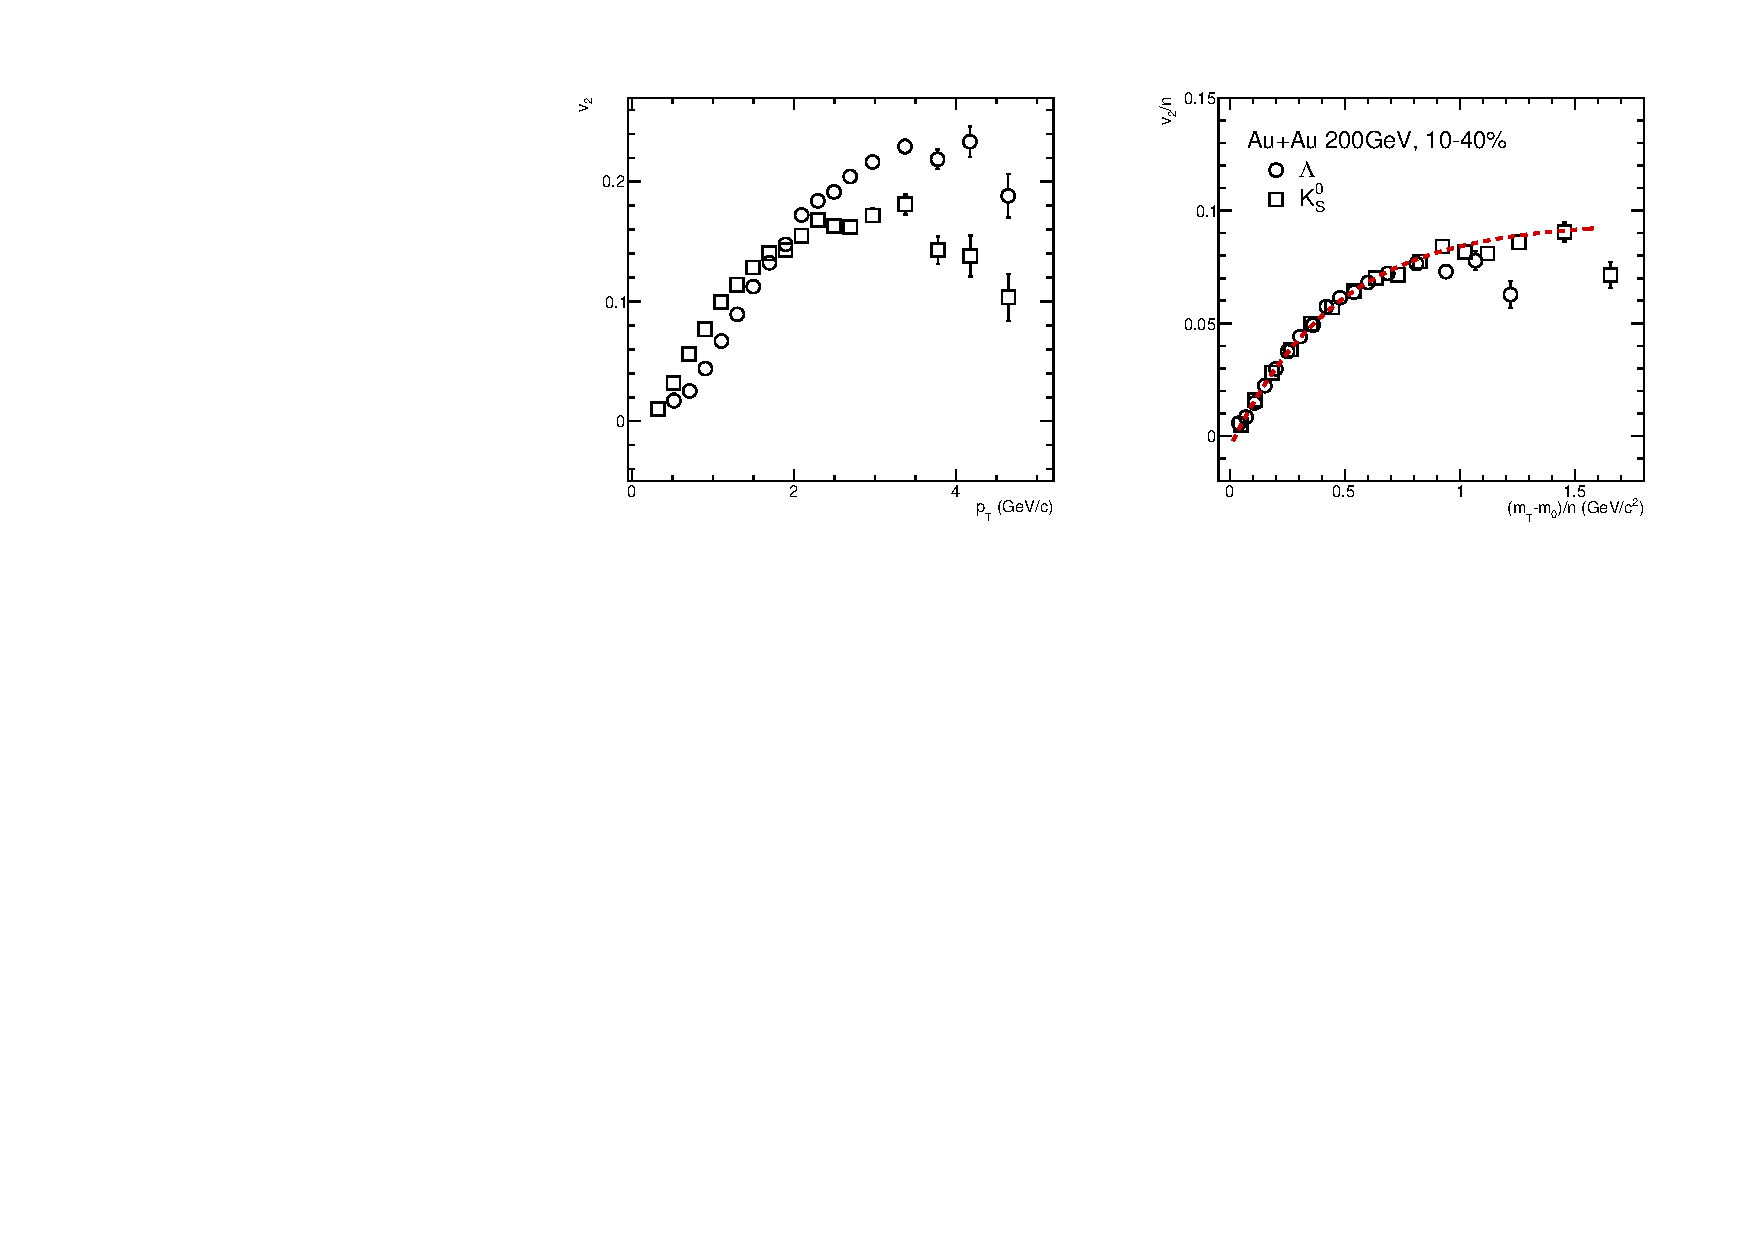
\includegraphics[scale=0.5]{FXT3gev/chapter4/fig/lam_ks0_v2ncq.pdf}
    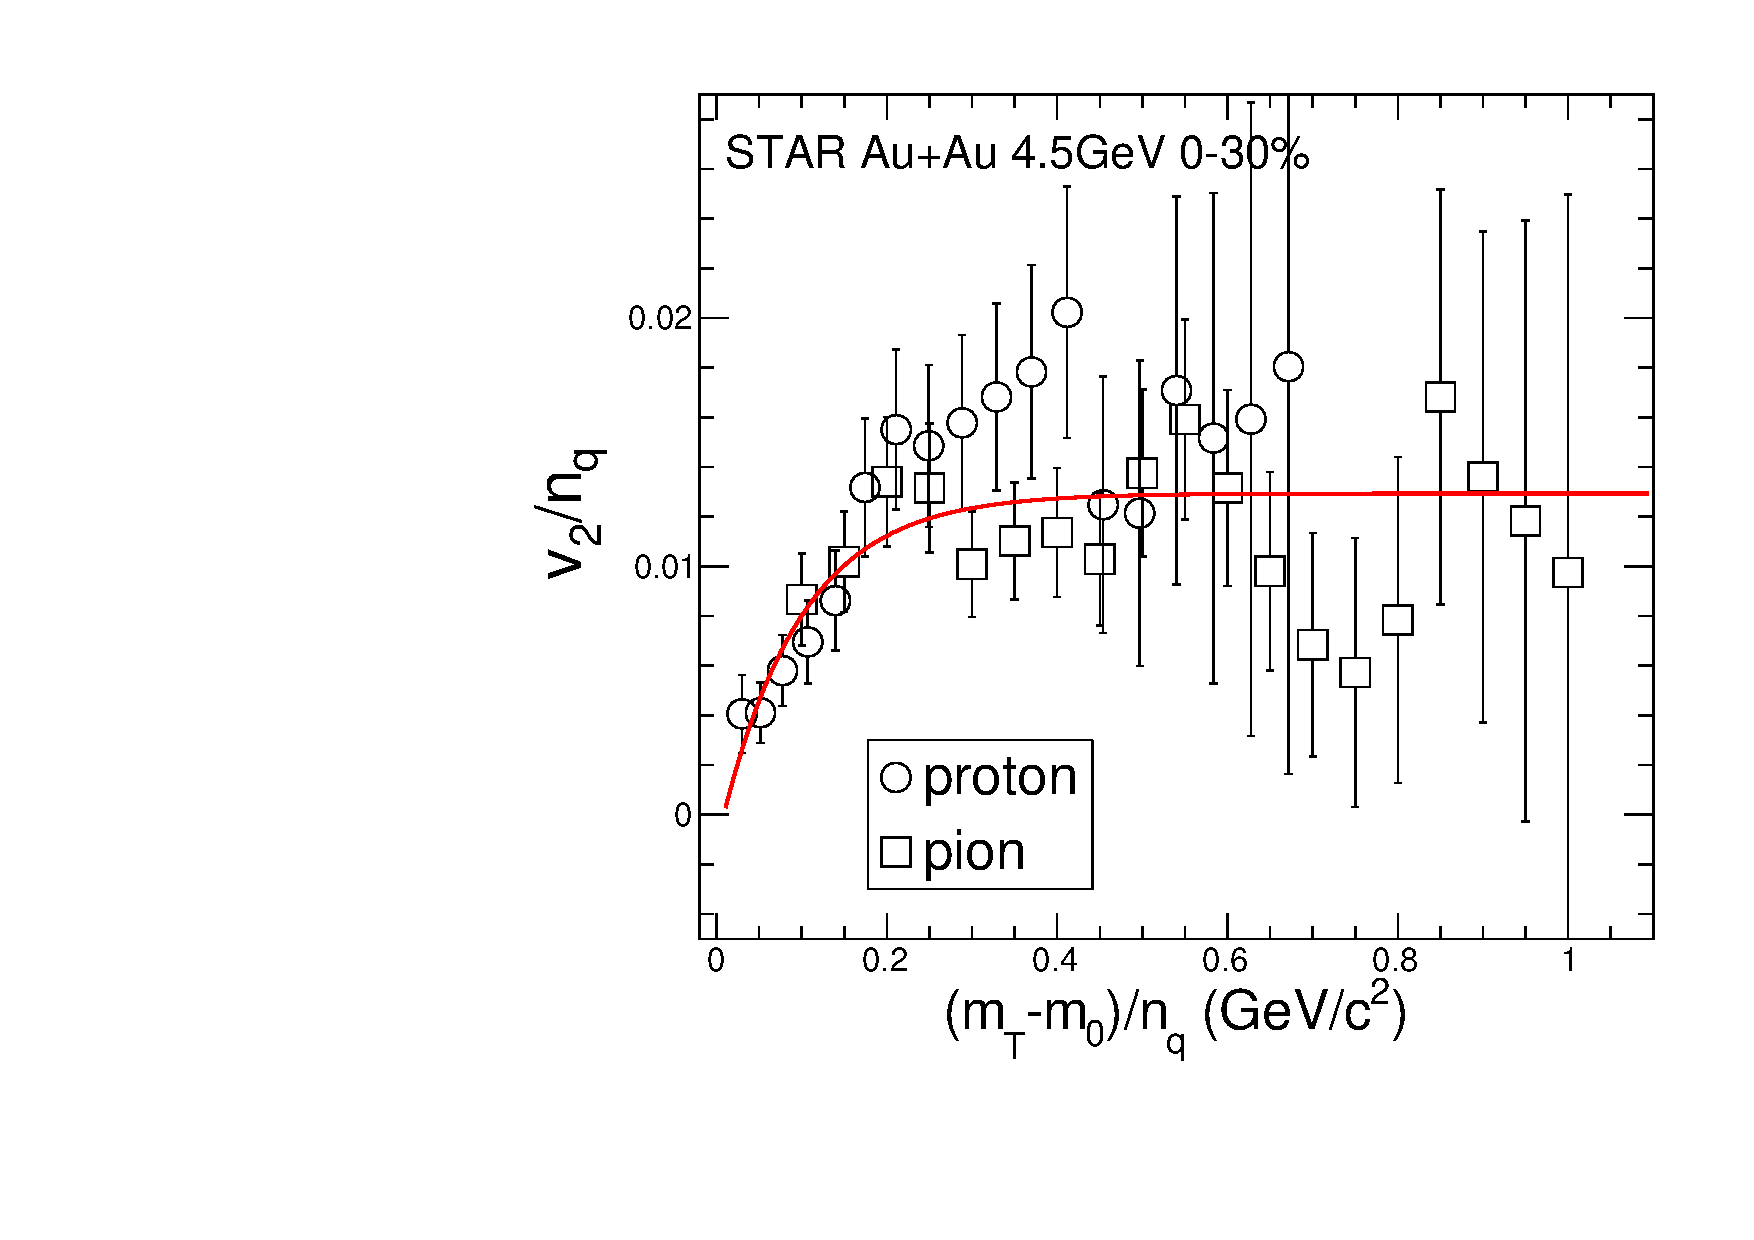
\includegraphics[scale=0.25]{FXT3gev/chapter4/fig/4_5GeV_ncq.pdf}
    \caption{Fitting to STAR data from 200-4.5 GeV in 10-40\% centrality.}
    \label{fig:v2pt_ncq_fit}
\end{figure} 

\clearpage
\newpage

\subsection{$p_{T}$ integrated $v_{2}$}

In order to compare the $p_{T}$ integrated $v_{2}$ at 3GeV with world data. In this chapter, we talk about the calculation of $p_{T}$ integrated $v_{2}$.

The $p_{T}$ integrated $v_{2}$, is also average $v_{2}$, over certained $p_{T}$ region. We denote the average $v_{2}$ as $<v_{2}>$, it can be calculated using formula \ref{ave_v2}. Where the $dN/dp_{T}$ is the transverse momentum distribution and $v_{2}(p_{T})$ is measured differential $v_{2}$ as a function of $p_{T}$. Weighting by the number of particles, we can calculate the average $v_{2}$ ($<v_{2}>$) in the centained $p_{T}$ range.

\begin{equation}
    <v_{2}> = \frac{\sum_{i} dN^{i}/dp_{T}*v_{2}^{i}(p_{T})}{\sum_{i}dN^{i}/dp_{T}}
    \label{ave_v2}
\end{equation}

Figure \ref{fig:dndpt_v2pt_proton} shows the proton $dN/dp_{T}$ distribution and differential $v_{2}$ as a function of $p_{T}$ in 10-40\% at 3GeV. From these distribution associated with formula \ref{ave_v2}, we can calculate proton $<v_{2}>$ in $p_{T}$ range [0.4,2.0] GeV/c and apply the same procedure to calculate $\pi^{\pm}$ $<v_{2}>$ in the $p_{T}$ range [0.2, 1.6] GeV/c.

Figure \ref{fig:v2_energy} shows the measured $p_{T}$ integrated $v_{2}$ as a function of collision energy. The STAR data points are proton and pion $v_{2}$ from BES-I energy 10-40\% and 4.5GeV 0-30\% \cite{Adam:2020pla}. The other data points shown are from FOPI \cite{Andronic:2004cp}, E895 \cite{Pinkenburg:1999ya}, and E877 \cite{Voloshin:1997rs}. As we can see, the new results at 3GeV from STAR are well agree with world data trend.

\begin{figure}
    \centering
    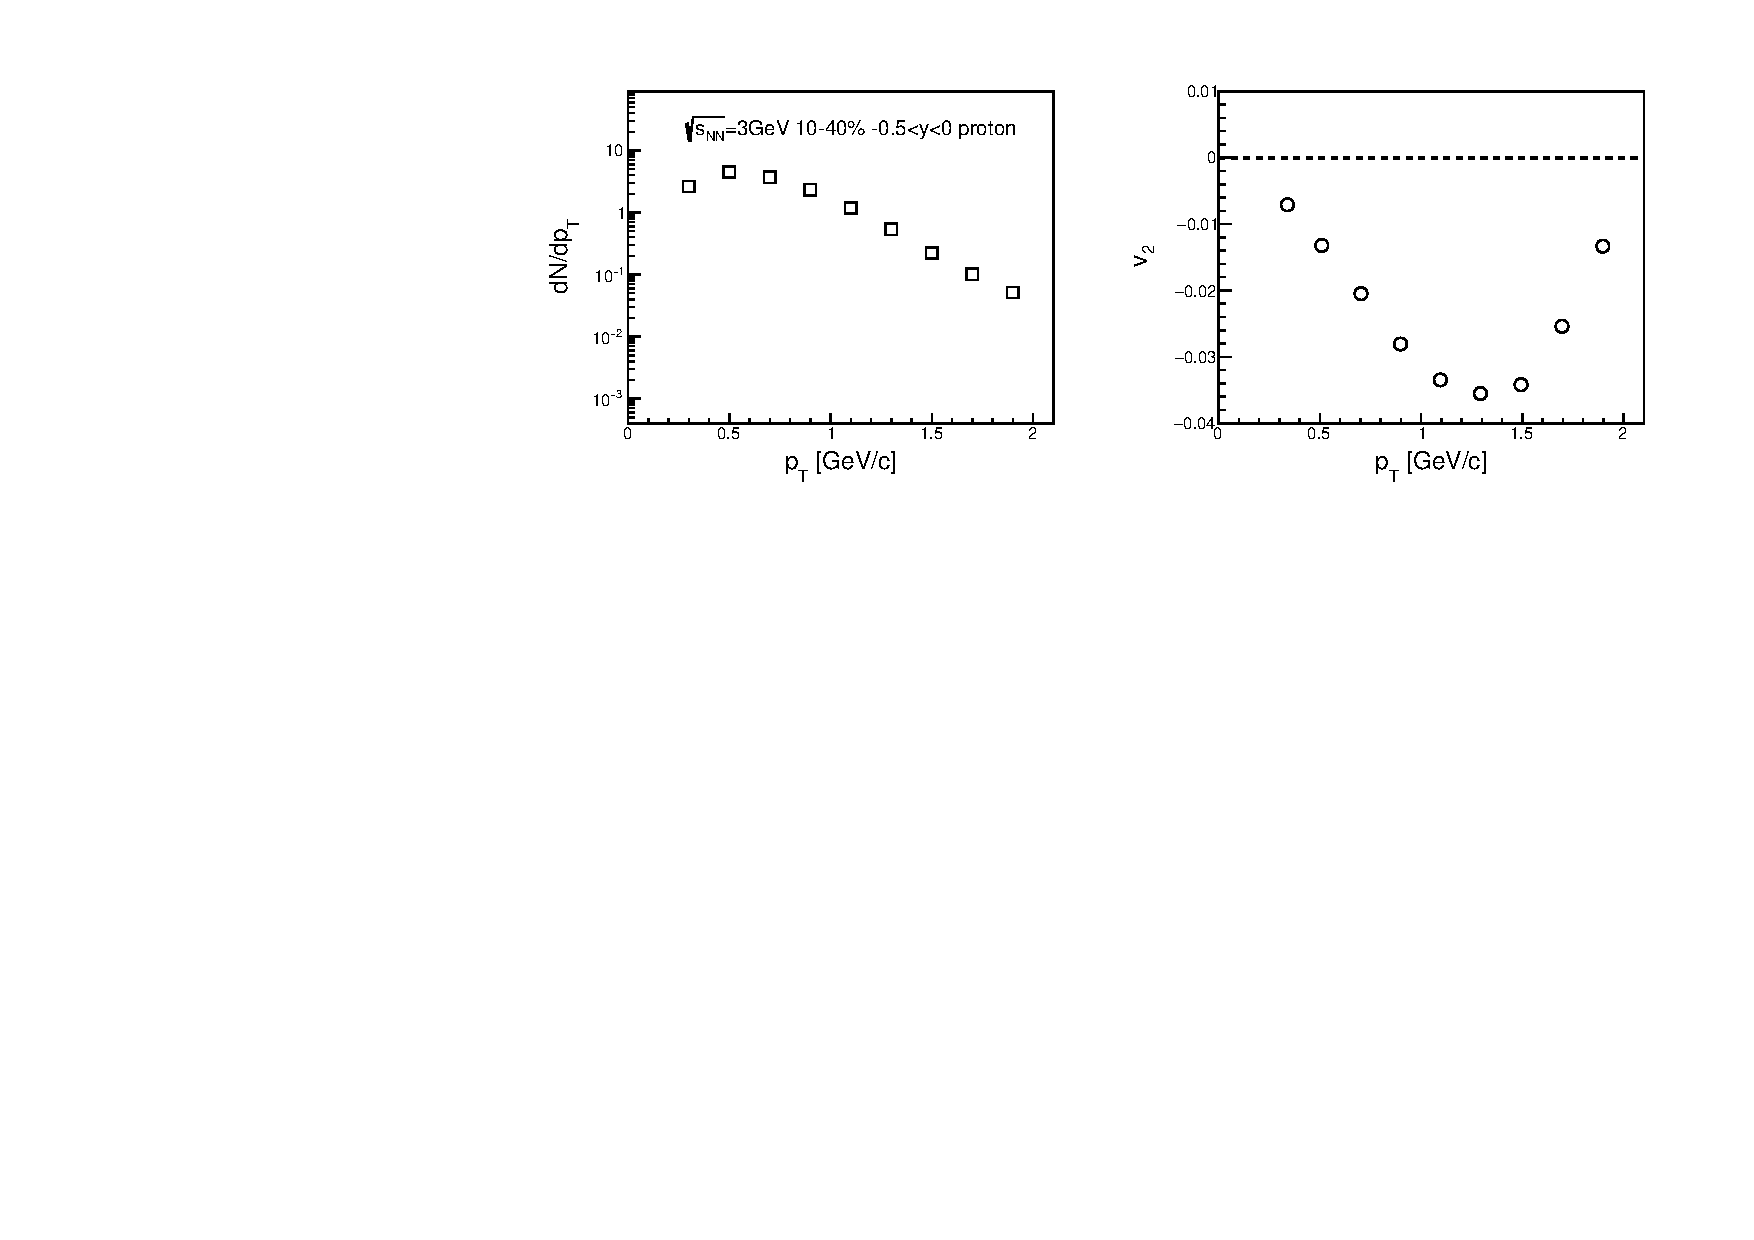
\includegraphics[scale=0.6]{FXT3gev/chapter4/fig/v2integral_proton.pdf}
    \caption{(Left) $dN/dp_{T}$ distribution for proton in 10-40\%. (Right) Differential $v_{2}$ as a function of $p_{T}$ for proton in 10-40\%.}
    \label{fig:dndpt_v2pt_proton}
\end{figure}

\begin{figure}
    \centering
    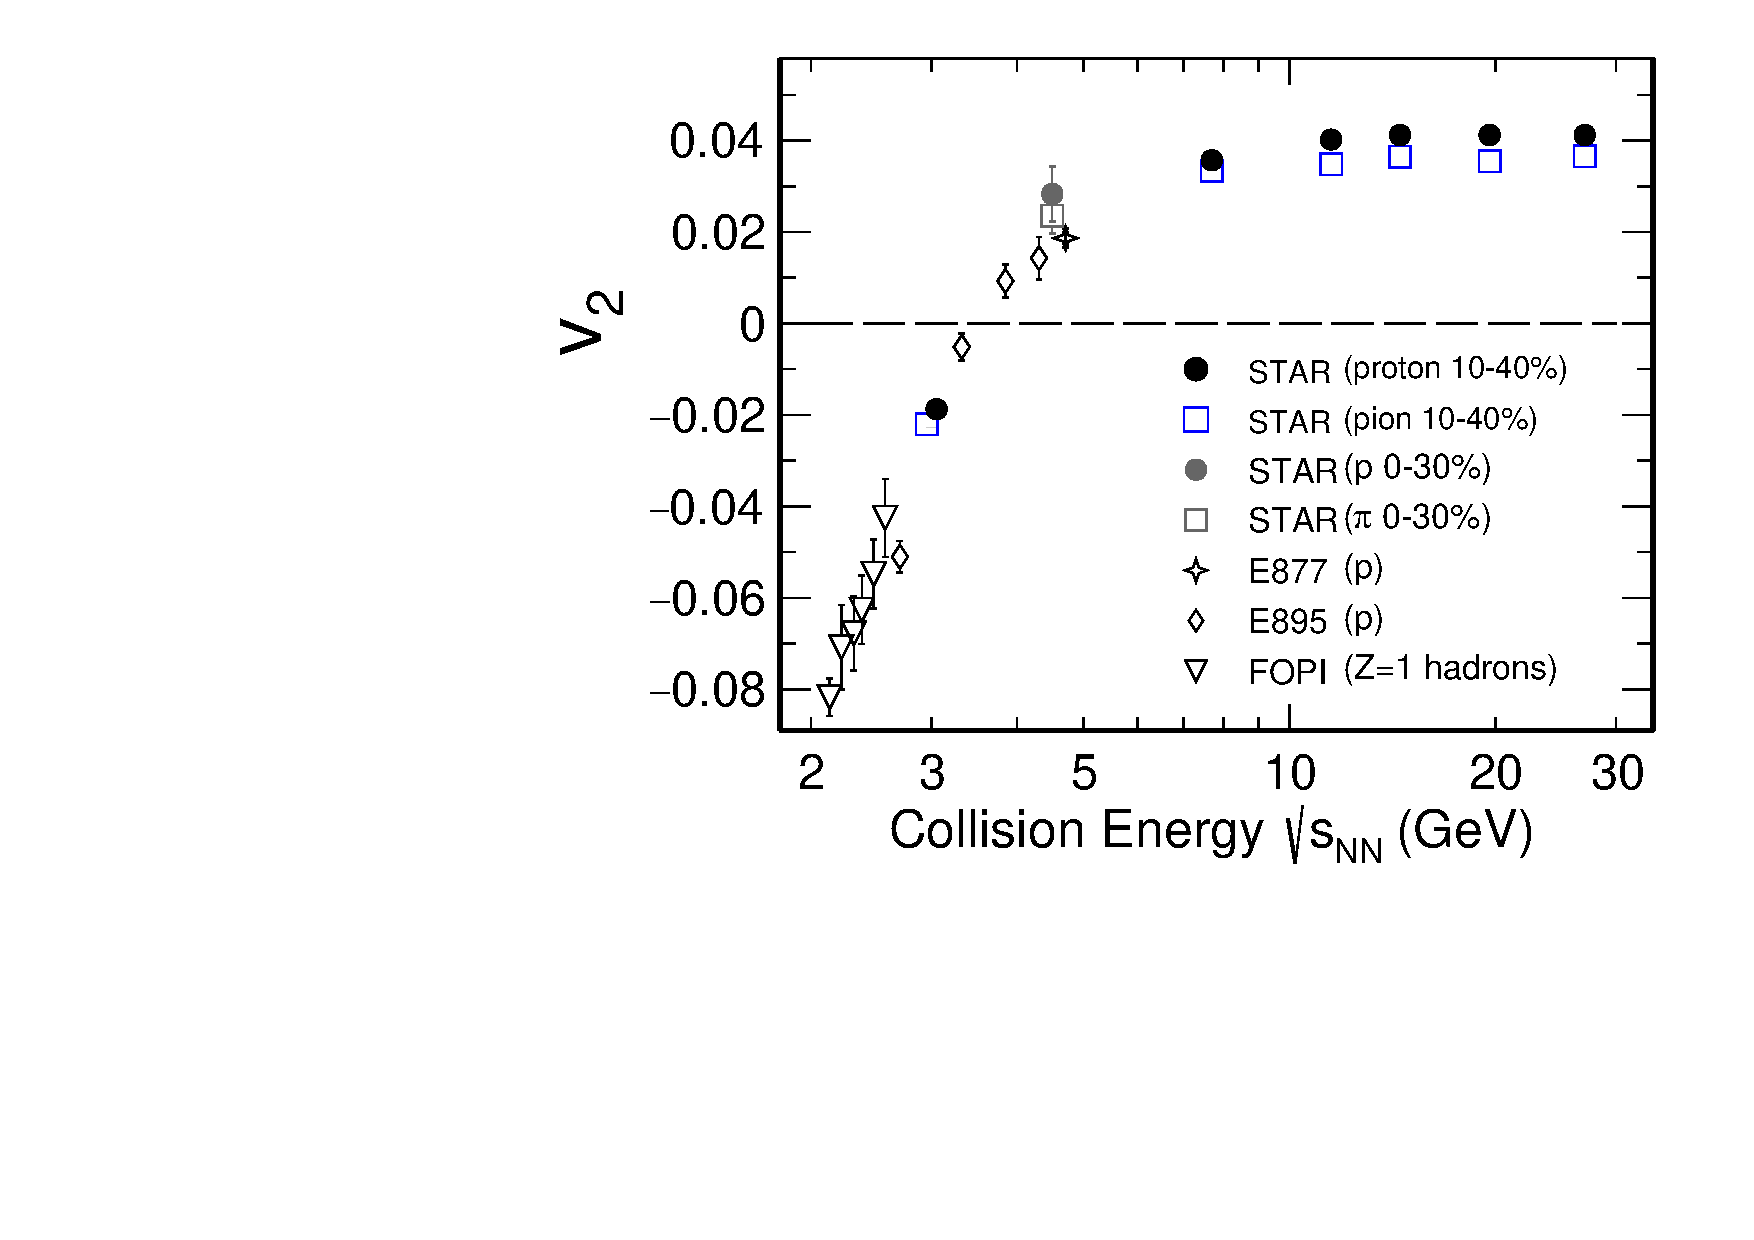
\includegraphics[scale=0.5]{FXT3gev/chapter4/fig/v2_energy.pdf}
    \caption{$p_{T}$ integrated $v_{2}$ for proton, pion or Z=1 hadrons as a function of collision energy. The STAR data point are proton and pion $v_{2}$ from BES-I 10-40\%, and 4.5GeV 0-30\%, and 3GeV 10-40\%. The other data are shown from FOPI, E985, E877.}
    \label{fig:v2_energy}
\end{figure}

\clearpage
\newpage
\subsection{Directed flow measurements}

Directed flow measurement of identified particles from STAR has been performed from 200GeV down to 4.5GeV \cite{Adamczyk:2014ipa, Adamczyk:2017nxg, Adam:2020pla}. The non-monotonic collision energy dependence proton  directed flow has been argued for a evidence of softenest point of equation of state \cite{Hung:1994eq, Konchakovski:2014gda, Nara:2016phs}. While other particle's $v_{1}$ are all negative. From previous AGS E895 measurements of proton directed flow $v_{1}$, we know the proton and $\Lambda$ $v_{1}$ are positive when collision energy $\sqrt{s_{NN}} <$ 10GeV and increase with collision energy decreases \cite{Liu:2000am}.  

In this analysis at 3GeV, we present $\pi^{\pm}, K^{\pm}, K^{0}_{S}, proton, \Lambda, \phi$ $v_{1}$ in 10-40\% centrality and compared to that from STAR high energy
 in figure \ref{fig:v1_energy}, As we can see, the proton and $\Lambda$ results are consistent with the energy trend and pions $v_{1}$ stays negative. But for the first time that the kaon and $\phi$ $v_{1}$ are found to be positive which is consistent with a change of equation of state. At 3Gev, it has been reached to high baryon density region, the $K^{+}$ will be associated production with $\Lambda$ and might follow collective behavior with $\Lambda$.


\begin{figure}
    \centering
    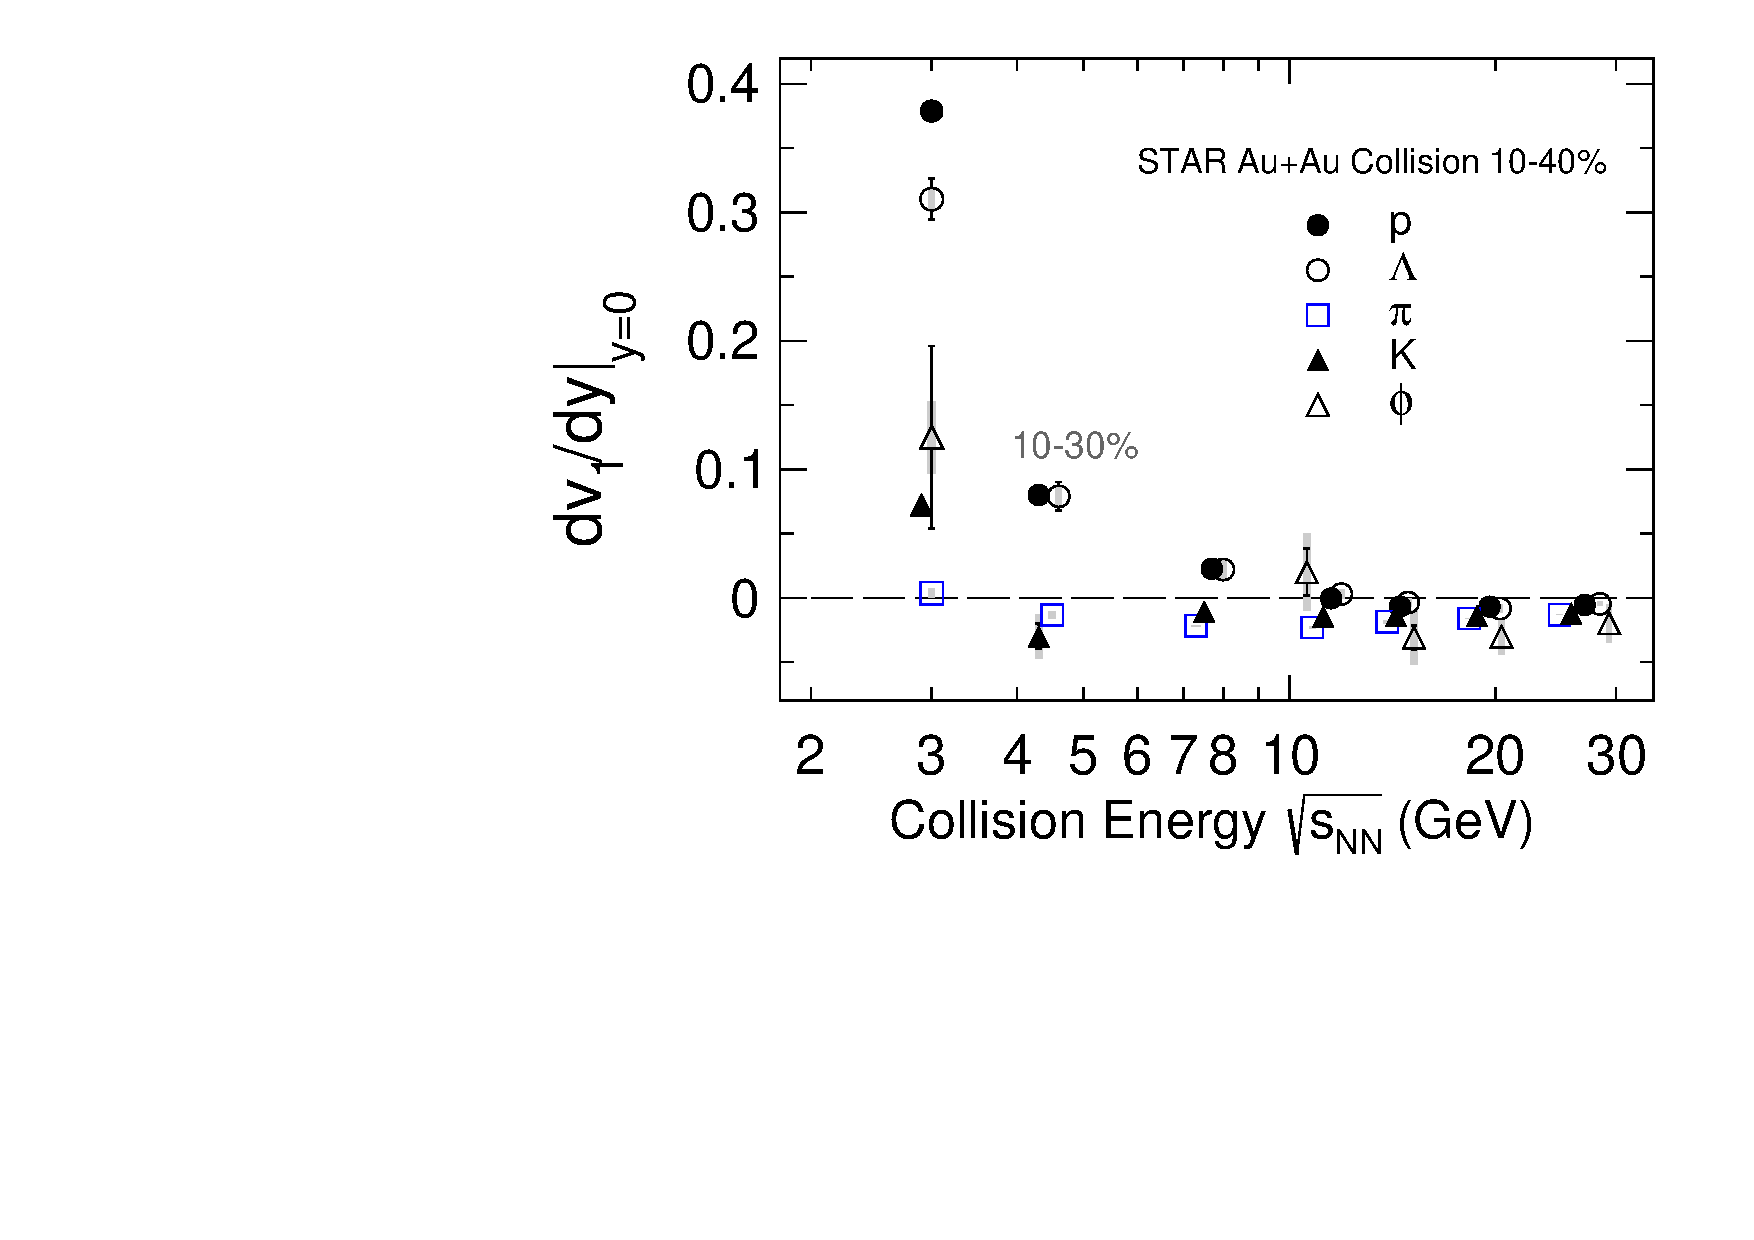
\includegraphics[scale=0.5]{FXT3gev/chapter4/fig/v1_energy.pdf}
    \caption{Collision energy dependence of directed flow $v_{1}$ slope for pion, kaon, proton, $\Lambda$ and $\phi$ in 10-40\% or 10-30\% from STAR.} 
    \label{fig:v1_energy}
\end{figure}

\subsection{Combination Results}

In this analysis, the $v_1$ results between positive and negative particle are combined for both pions and kaons, as the difference among them are very small. 
The method for combining these results are listed below: firstly the weight factor is calculated by the inverse of statistics error square. Then we combined results and error are calculated by weighting the weight factor, the similar way for kaons analysis.

\begin{equation}
    w (\pi^{+}) = \frac{1}{error_{stat}(\pi^{+})} \qquad
    w (\pi^{-}) = \frac{1}{error_{stat}(\pi^{-})}
\end{equation}

\begin{equation}
    v_{1}(\pi) = \frac{v_{1}(\pi^{+})*w(\pi^{+}) + v_{1}(\pi^{-})*w(\pi^{-})}{w(\pi^{+})+w(\pi^{-})}
\end{equation}
\begin{equation}
    error_{stat}(\pi) = \sqrt{1/(w(\pi^{+})+w(\pi^{-}))}
\end{equation}
\begin{equation}
    error_{sys}(\pi) = \frac{error_{sys}(\pi^{+})*w(\pi^{+}) + error_{sys}(\pi^{-})*w(\pi^{-})}{w(\pi^{+})+w(\pi^{-})}
\end{equation}



















